\documentclass[tikz,border=3mm]{standalone}
\usepackage{tikz}
\usetikzlibrary{angles,quotes,calc,intersections}
\begin{document}
% TikZ 1
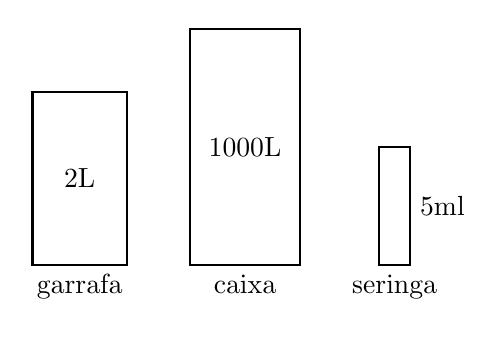
\begin{tikzpicture}[scale=1]
\draw[thick] (0,0) rectangle (1.2,2.2); \node at (.6,1.1) {$2\mathrm{L}$};
\draw[thick] (2,0) rectangle (3.4,3); \node at (2.7,1.5) {$1000\mathrm{L}$};
\draw[thick] (4.4,0) rectangle (4.8,1.5); \node[right] at (4.8,.75) {$5\mathrm{ml}$};
\node[below] at (.6,0) {garrafa}; \node[below] at (2.7,0) {caixa}; \node[below] at (4.6,0) {seringa};
\end{tikzpicture}
\hspace{1cm}
% TikZ 2
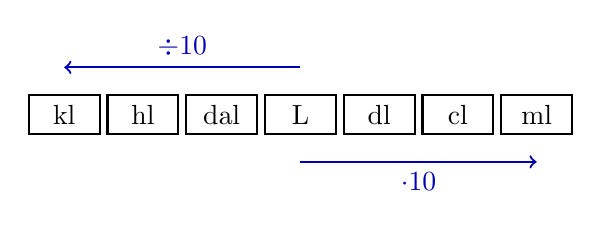
\begin{tikzpicture}[scale=1]
\foreach \x/\unit in {0/kl,1/hl,2/dal,3/L,4/dl,5/cl,6/ml}{
  \draw[thick] (\x,0) rectangle +(0.9,0.5);
  \node at (\x+.45,.25) {$\mathrm{\unit}$};
}
\draw[->,blue!70!black,thick] (3.45,-.35)--(6.45,-.35) node[midway,below] {$\cdot 10$};
\draw[->,blue!70!black,thick] (3.45,.85)--(.45,.85) node[midway,above] {$\div 10$};
\end{tikzpicture}

\vspace{1cm}

% TikZ 3
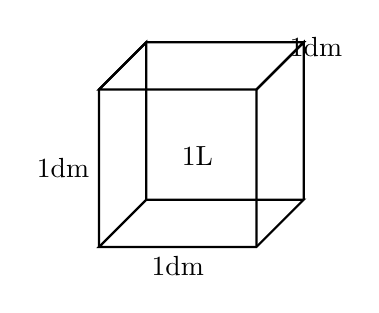
\begin{tikzpicture}[scale=1]
\draw[thick] (0,0)--(2,0)--(2.6,.6)--(.6,.6)--cycle;
\draw[thick] (0,0)--(0,2)--(.6,2.6)--(.6,.6);
\draw[thick] (2,0)--(2,2)--(2.6,2.6)--(2.6,.6);
\draw[thick] (0,2)--(2,2)--(2.6,2.6)--(.6,2.6)--cycle;
\node[below] at (1,0) {$1\mathrm{dm}$};
\node[left] at (0,1) {$1\mathrm{dm}$};
\node[above right] at (2.3,2.3) {$1\mathrm{dm}$};
\node at (1.25,1.15) {$1\mathrm{L}$};
\end{tikzpicture}
\end{document}
